\chapter{Cryptography in the TLS protocol}

\section{SSL/TLS Protocol}
\label{tls_proto}

\begin{figure}[!ht]
\centering
%\frame{
% trim: left, bottom, right, up
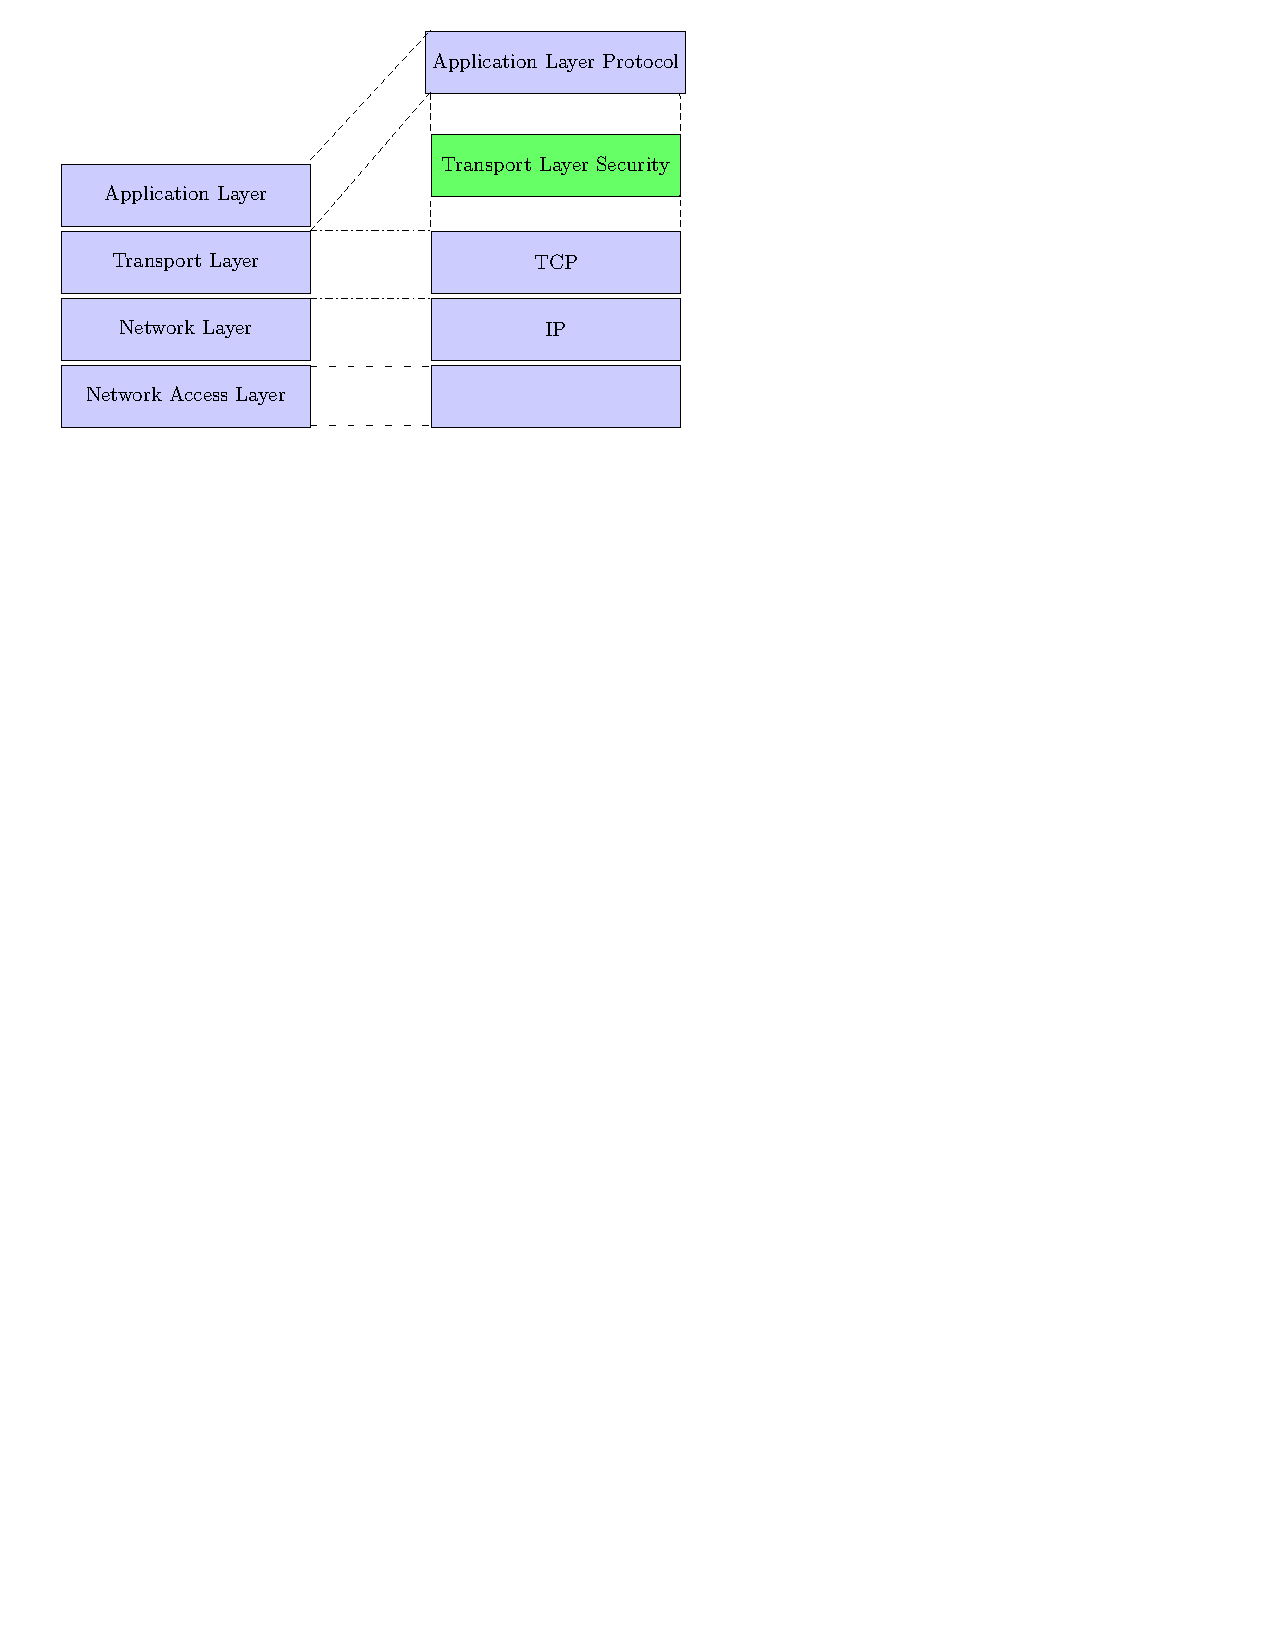
\includegraphics[trim=0cm 20.5cm 8cm 0cm]{figures/tls_osi.pdf}
\caption{TLS protocol in OSI model}
\label{fig:osi}
%}
\end{figure}

The Transport Layer Security (TLS) \cite{RFC5246}  provides communication
security, privacy and data integrity, over the Internet. Through this protocol two communicating peers
can communicate in a way which that is designed to prevent eavesdropping, tampering, or message forgery.
The TLS protocol is situated between the Application Layer and the Transport
Layer (e. g. TCP \cite{RFC0793}) in OSI model (see figure \ref{fig:osi}).

The protocol is composed of five layers (see figure
\ref{fig:tls_handshake}):

\begin{enumerate}[noitemsep]
  \item Handshake Protocol\newline
  Allows the two communicating peers (server and client) to
authenticate each other and to negotiate a cipher suite (see section
\ref{tls_ciph_suite}) and a compression method to transmit data.
  \item Change Cipher Spec Protocol\newline
  Allows to the communicating peers to signal a change of the ciphering
  strategy.
  \item Alert Protocol\newline
  Allows the communicating peers to signal potential problems and to exchange
  corresponding alert messages.
  \item Application Data Protocol\newline
  Is used for the secure transmission of application data
  \item Record Protocol\newline
  Is used for encapsulation of higher-layer protocol data,
such as TCP in case of the TCP/IP protocol \cite{RFC0793}.
It provides connection security with two basic properties:
\begin{enumerate}[noitemsep]
  \item Private connection, through symmetric cryptography algorithms (see
  section \ref{intro_sym_cipher})
  \item Reliable connection, through Message authentication Code (MAC) (see
  section \ref{intro_mac}) 
\end{enumerate}
\end{enumerate}

\begin{figure}[!ht]
\centering
%\frame{
% trim: left, bottom, right, up
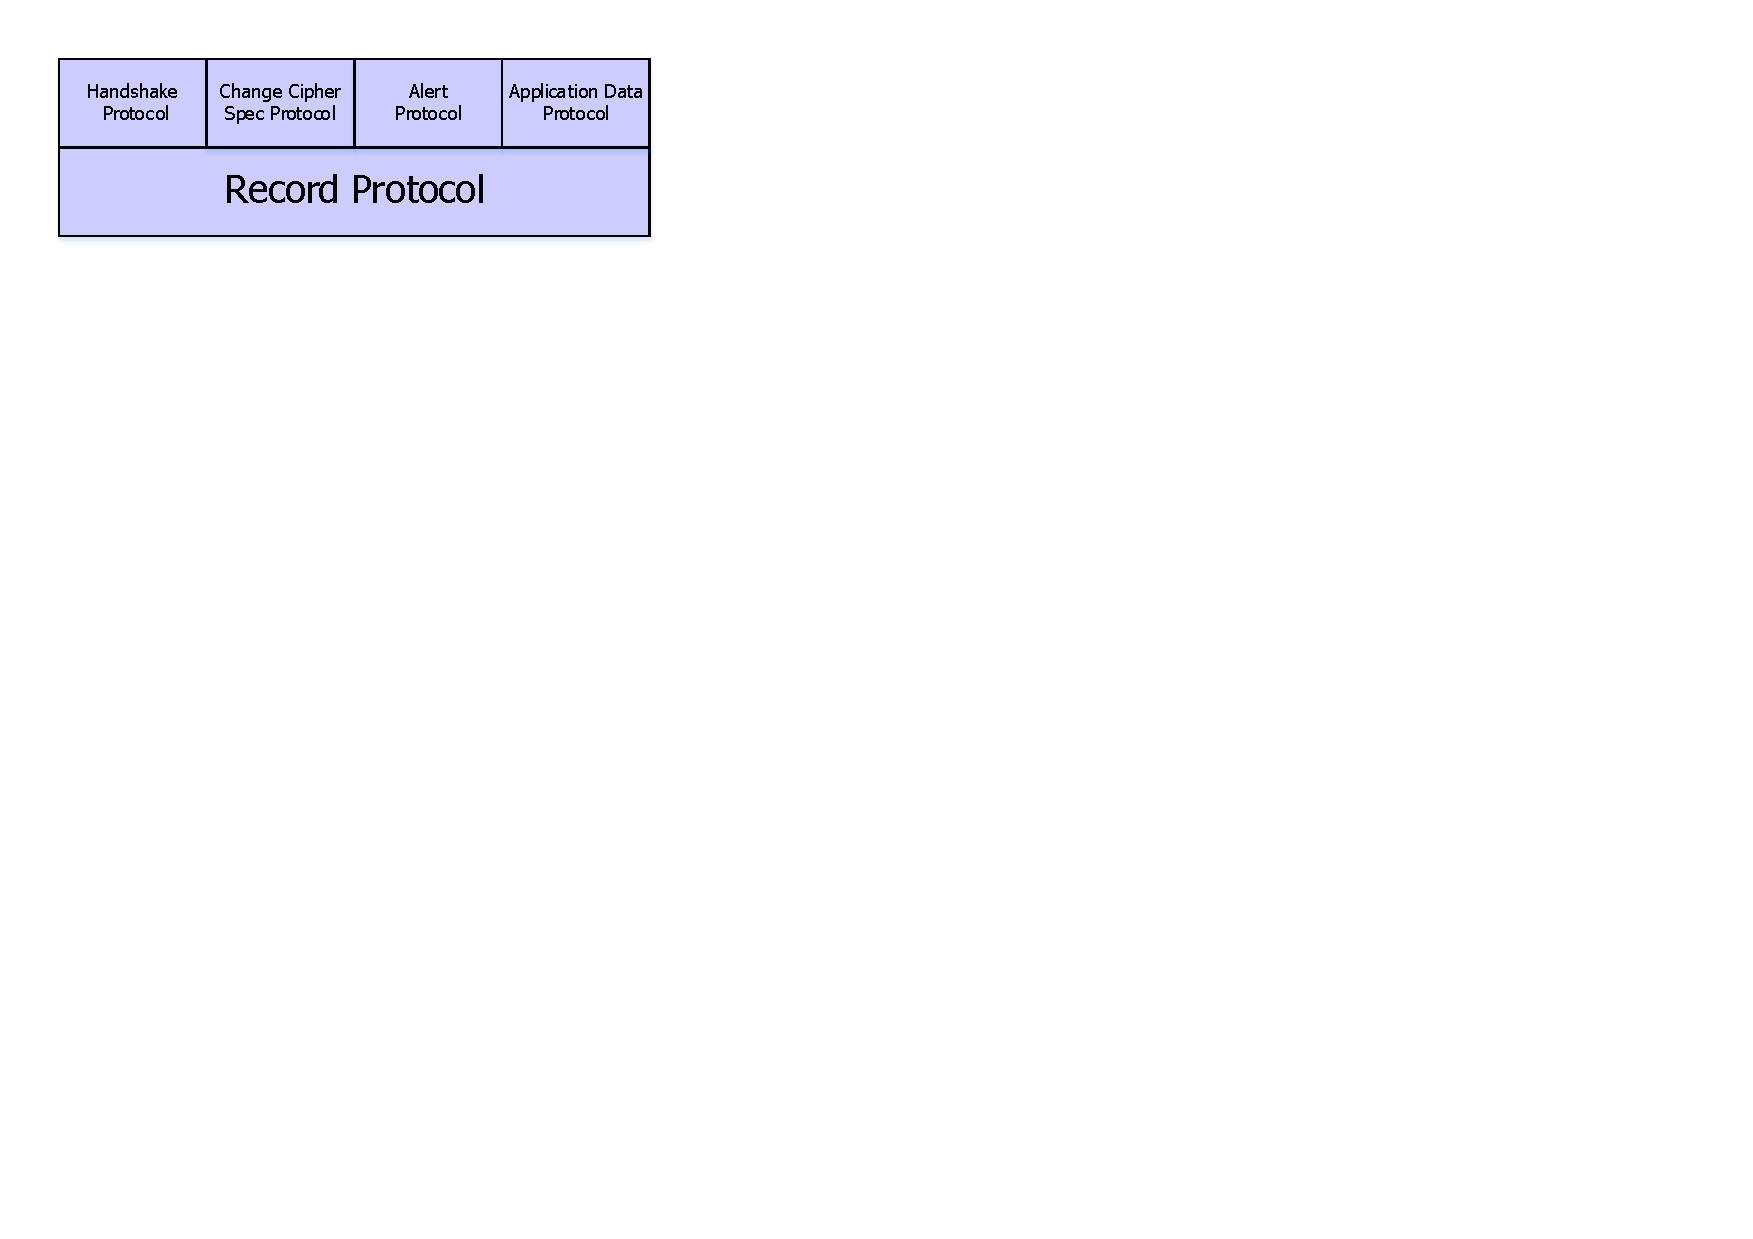
\includegraphics[trim=0cm 17cm 18cm 0cm]{figures/tls_handshake.pdf}
\caption{TLS Handshake Protocol}
\label{fig:tls_handshake}
%}
\end{figure}


\subsection{Cipher suites}
\label{tls_ciph_suite}
A cipher suite \cite{RFC5246} is used to cryptographically protect data in terms
of authenticity, integrity and confidentiality.
A cipher suite allows to know which key exchange, cipher and Message
Authentication Code (MAC) will be used during the session. Figure
\ref{fig:tls_ciph_suite} shows an example of a cipher suite.\newline
 

\begin{figure}[!ht]
\centering
% trim: left, bottom, right, up
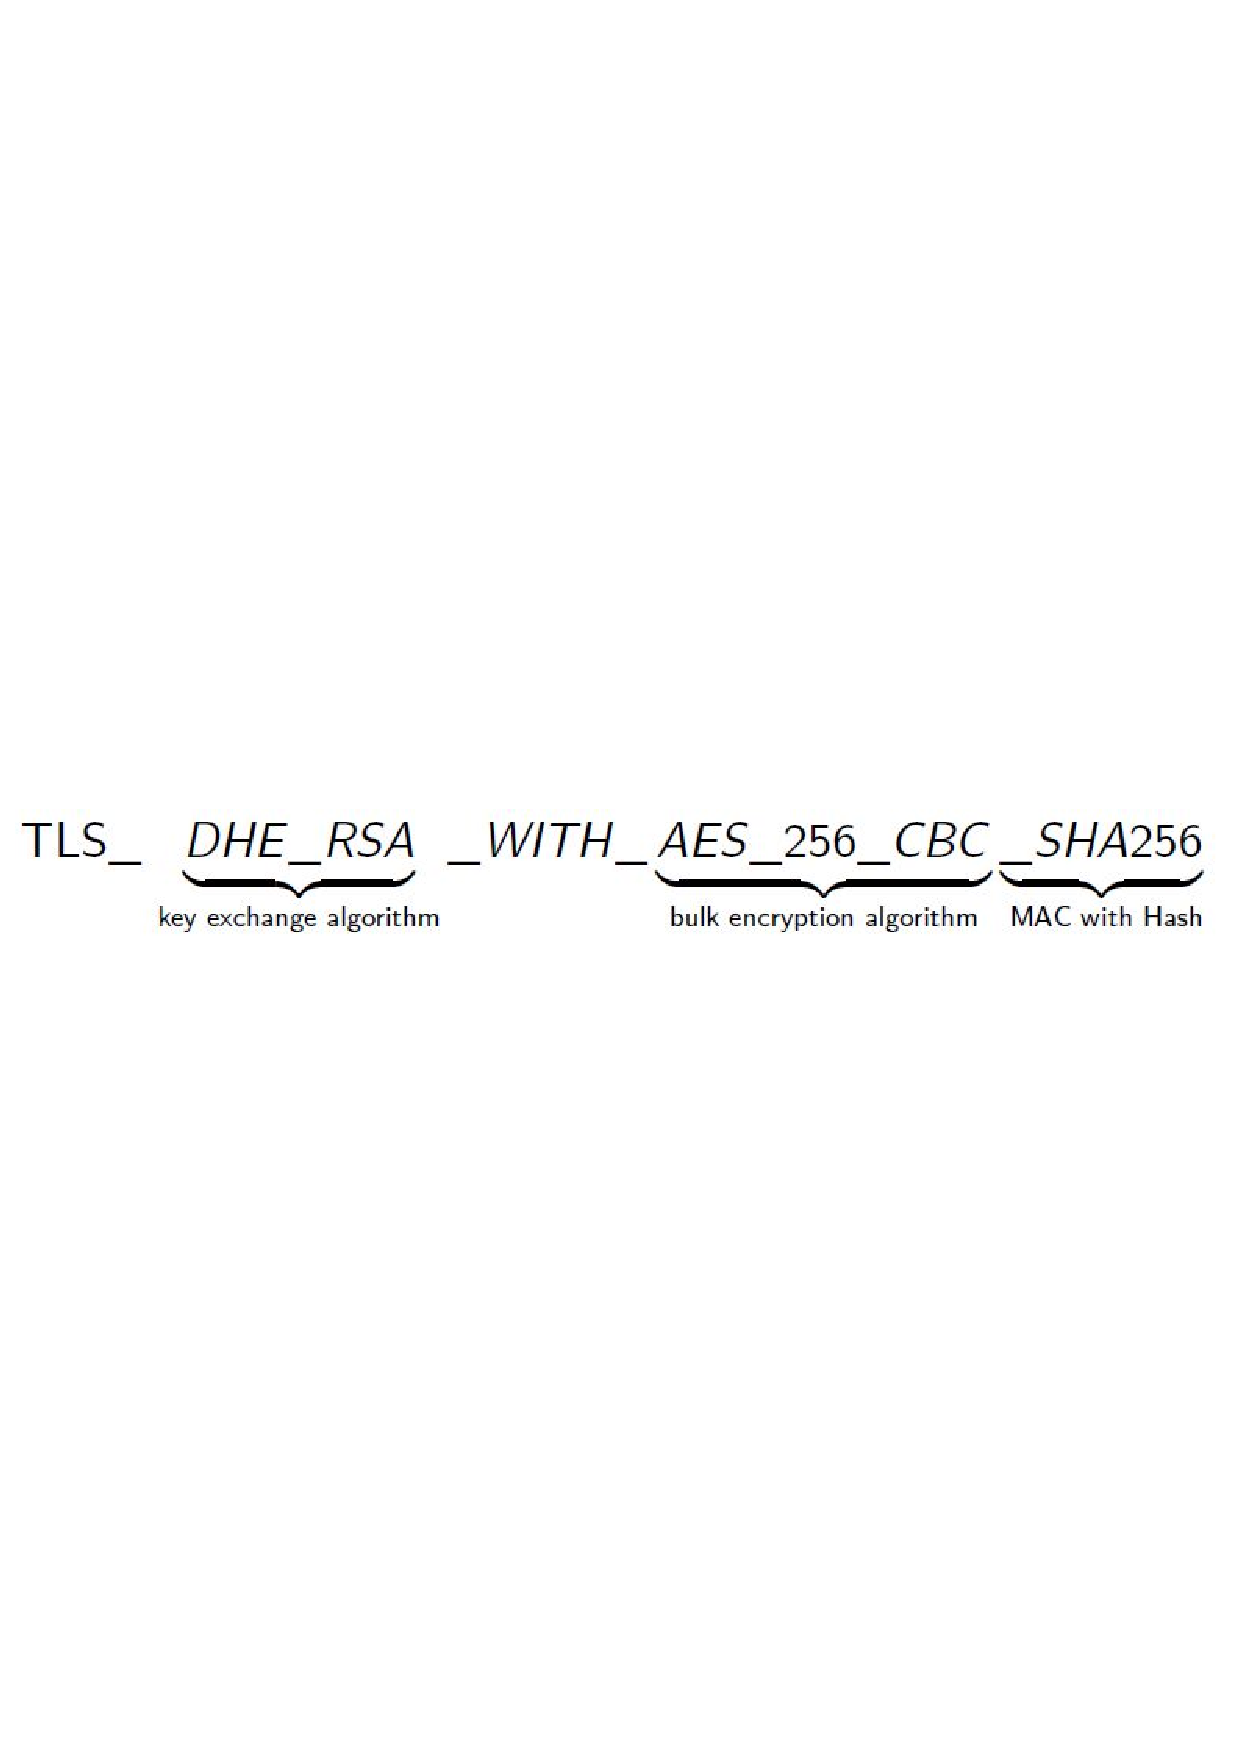
\includegraphics[trim=0cm 13.5cm 0cm 13.5cm,
height=1.75cm]{figures/tls_cipher_suite.pdf}
\caption{Example of a cipher suite}
\label{fig:tls_ciph_suite}

\end{figure}

\newpage

\section{Cryptographic parts in the Handshake Protocol}

This part describes step by step which cryptographic algorithms are used, how
they work and why these algorithms are used, for each step of the Handshake
Protocol \cite{RFC5246}.

\begin{figure}[!ht]
\centering
% trim: left, bottom, right, up
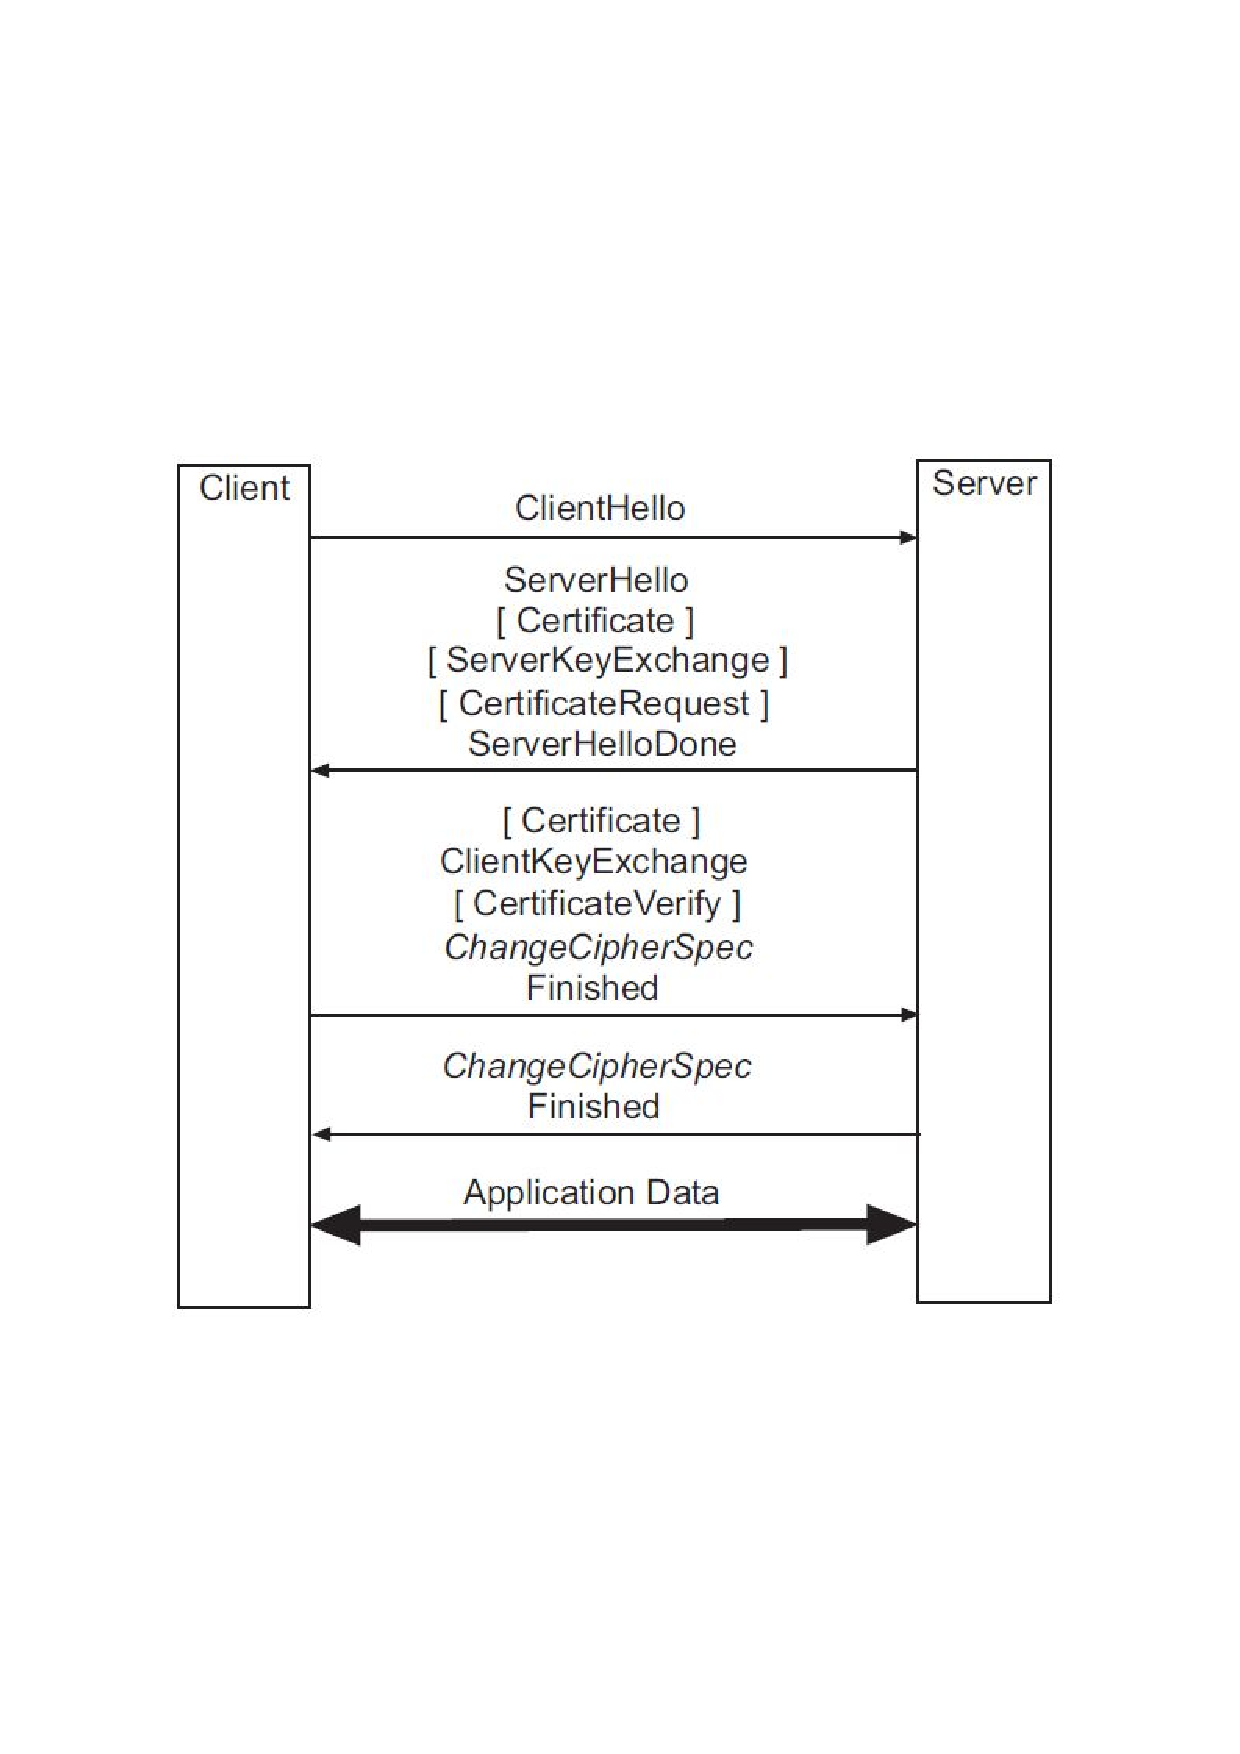
\includegraphics[trim=0cm 7cm 0cm 7cm,
height=9.5cm]{figures/tls_exg.pdf}
\caption{Handshake protocol (source \cite{book2})}
\label{fig:tls_exg}

\end{figure}

\subsection*{Client Hello}

A random number is generated as Client random number.

Creation of a hash function in the Client which will be used during the whole
communication.
Each received and transmitted data are added to this hash function, which allows
to be sure that the two peers have become the same data. The data of the Client
Hello are added to the hash function.

The cryptographic algorithms use in this message are:
\begin{itemize}[noitemsep]
  \item Random Number Generator (seed + generation of a random number)
  \item Hash algorithm (creation + update)
\end{itemize}


\subsection*{Server Hello}

Generation of a Server random number.
The cipher suite is chosen by the Server, which chooses with the list of cipher
suites sent by the Client in the Client Hello.

Creation of a hash function in the Server which will be used during the whole
communication.
Each received and transmitted data are added to this hash function, which allows
to be sure that the two peers have become the same data. 
The data from the Client Hello and of Server Hello are added to the hash
function of the Server and the data of the Server Hello is added to the hash
function of the Client too.

The cryptographic algorithms use in this message are:
\begin{itemize}[noitemsep]
  \item Random Number Generator (seed + generation of a random number)
  \item Hash algorithm (creation + update)
\end{itemize}

\subsection*{Certificate}
The certificate message is sent from the Server. It contains certificates which
each one contains public key certificates which contain public keys,
digital signatures and other informations.
A public key is extracted and used to verify a digital signature which
authenticates the server.
The Client can also use this public key to verify the digital signature from
the certificate and authenticates the Server.
This message is added to the Client and Server hash function.

The Client sends its certificates when a Certificate Request has been sent from
Server.

The cryptographic algorithm uses in this message is:
\begin{itemize}[noitemsep]
  \item Digital signature algorithm (verification)
  \item Hash algorithm (update)
\end{itemize}

\subsection*{Server Key Exchange}
The Server Key Exchange is sent when Diffie-Hellman or Elliptic Curve
Diffie-Hellman  is used as key exchange.
In this Server Key Exchange the domain parameters are sent, which are used to
generate the public key of the Client and of the Server.

The public key of the Server and the private key of the public key are used to
generate the secret key.

The data of the Server Key Exchange are added to the hash function of the Client
and the Server.

The cryptographic algorithms use in this message are:
\begin{itemize}[noitemsep]
  \item Diffie-Hellman/Elliptic Curve Diffie Hellman algorithm (Generation of
  key pair + calculation of the secret key)
  \item Hash algorithm (update)
\end{itemize}

\subsection*{Certificate Request}
The Certificate Request message is used when the Server wants the certificates
of the Client to authenticate it.
The certificate message is added to the hash function of the Client and the
Server.

Ony the hash algorithm (update) is used as a cryptographic algorithm for this
message.

\subsection*{Server Hello Done}
The Server Hello Done is only added to the hash function of the two peer.
Therefore is only the hash algorithm (update) used for this message.

\subsection*{Client Key Exchange}
If the RSA is used as key exchange, the premaster key is computed with the Client and Server random
number, sent in the Client Hello and Server Hello, with the HMAC function uses
in the PRF \cite{RFC5246}.
This premaster secret is encrypted with the public key of the Server, which is
extracted from the certificate coming from the Server Hello.
Only the Server which has the private key can decrypt this premaster key.

When the Server receives the Client Key Exchange, he computes the premaster key
too. He can compare its premaster key with this one decrypted from the Client
Key Exchange.

If the Diffie-Hellman or Elliptic Curve Diffie Hellman (ECDH) is used as key
exchange, the public key generates by the Client, with the domain parameters
send in the Server Key Exchange message, is sent to the Server.
Then the Server can compute the secret key too. 

The Client Key Exchange message is added to the hash function of the Client and
the Server

The cryptographic algorithms use in this message are:
\begin{itemize}[noitemsep]
  \item Hash-based Message Authentication Code (HMAC) algorithm (Generation)
  \item Diffie-Hellman / Elliptic Curve Diffie-Hellman algorithm (Calculation of
  the secret key) if Diffie-Hellman / Elliptic Curve Diffie-Hellman is used as
  key exchange
  \item RSA algorithm (Decryption) if RSA is used as key exchange
  \item Hash algorithm (update)
\end{itemize}

\subsection*{Certificate Verify}
The Client sents a digital signature, which has been done with the private key
of the Client, to the Server, so the Server can authenticates the Client with
the public extracts from the Client certificates.
This message is added to the Client and Server hash function.

The hash algorithms use in this message are:
\begin{itemize}[noitemsep]
  \item Digital signature algorithm (Generation and verification)
  \item Hash algorithm (update)
\end{itemize}


\subsection*{Change Cipher Spec}
This message allows to the communicating peers to signal transitions in
ciphering strategies, meaning that the key exchange will be the symmetric one
chooses in the cipher suite.
No cryptographic algorithms are used for this message.


\subsection*{Finish}
This message allows to the two peers to verify that the key exchange and
authentications have been successful. The digest of the hash function uses since
the beginning of the communication is computed. A Message Authentication Code is
computed with the secret key.
The two results are encrypted with the secret key and the symmetric algorithm
chooses in the cipher suite.
The other peer can then decrypt the message with the secret key and compare
the results. If the results are the same, it means that there are communicated
together since the beginning, without disturbing. If the results are different,
it means that there are security problems, as eavesdropping, tampering, or
message forgery, and an Alert message is then sent. The message is added to the
hash function of the two peers.

The cryptographic algorithms use in this message are:
\begin{itemize}[noitemsep]
  \item Symmetric cipher algorithm (encryption and decryption)
  \item Message Authentication Code (generation)
  \item Hash algorithm (computing digest, update)
\end{itemize}



\subsection*{Application Data}
In this step, data can be transmitted over an insecure network without potential
security problems.
The data is signed with a Message Authentication Code (MAC) with the secret
key.
The data and the MAC are encrypted and decrypted with the secret key and the
symmetric algorithm chooses in the cipher suites.

The cryptographic algorithms use in this message are:
\begin{itemize}[noitemsep]
  \item Message Authentication Code (generation)
  \item Symmetric cipher algorithm (encryption and decryption)
\end{itemize}
